\begin{figure*}[t]
\centering
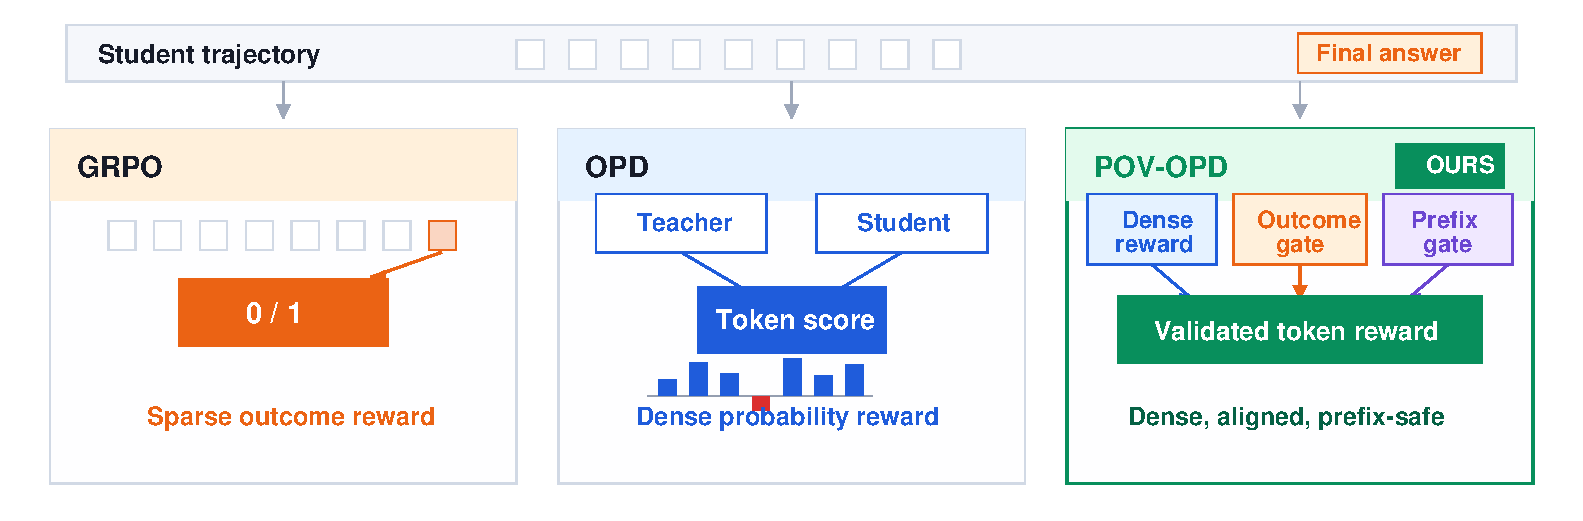
\includegraphics[width=\textwidth]{figures/pov_comparison.pdf}
\caption{Credit assignment on the same student rollout. GRPO group-normalizes the terminal verifier reward and broadcasts one scalar within each trajectory, whereas OPD provides signed dense teacher--student gaps without validating them. POV-OPD turns the terminal result into a local outcome-validity weight, detects sustained prefix drift from windowed teacher excess surprisal using CUSUM, and boosts only aligned candidates that remain well supported by the teacher. The sampled-token example at the bottom shows how the three nonnegative weights preserve, remove, cap, or decay each dense OPD signal without reversing its sign.}
\label{fig:pov_comparison}
\end{figure*}
